%%%%%%%%%%%%%%%%%%%%%%%%%%%%%%%%%%%%%%%%%%%%%%%%%%%%%%%%%%%%%%%%%%%%%
%
% CSCI 1430 Written Question Template
%
% This is a LaTeX document. LaTeX is a markup language for producing documents. 
% You will fill out this document, compile it into a PDF document, then upload the PDF to Gradescope. 
%
% To compile into a PDF on department machines:
% > pdflatex thisfile.tex
%
% If you do not have LaTeX, your options are:
% - VSCode extension: https://marketplace.visualstudio.com/items?itemName=James-Yu.latex-workshop
% - Online Tool: https://www.overleaf.com/ - most LaTeX packages are pre-installed here (e.g., \usepackage{}).
% - Personal laptops (all common OS): http://www.latex-project.org/get/ 
%
% If you need help with LaTeX, please come to office hours.
% Or, there is plenty of help online:
% https://en.wikibooks.org/wiki/LaTeX
%
% Good luck!
% The 1430 staff
%
%%%%%%%%%%%%%%%%%%%%%%%%%%%%%%%%%%%%%%%%%%%%%%%%%%%%%%%%%%%%%%%%%%%%%

\documentclass[11pt]{article}

\usepackage[english]{babel}
\usepackage[utf8]{inputenc}
\usepackage{amssymb}
\usepackage{xcolor}
\usepackage[colorlinks = true,
            linkcolor = blue,
            urlcolor  = blue]{hyperref}
\usepackage[a4paper,margin=1.5in]{geometry}
\usepackage{stackengine,graphicx}
\usepackage{fancyhdr}
\setlength{\headheight}{15pt}
\usepackage{microtype}
\usepackage{times}
\usepackage[shortlabels]{enumitem}
\setlist[enumerate]{topsep=0pt}
\usepackage{amsmath}
\usepackage{framed}
\usepackage{mdframed}
\usepackage{xcolor}
\usepackage[most]{tcolorbox}

% a great python code format: https://github.com/olivierverdier/python-latex-highlighting
\usepackage{pythonhighlight}

\usepackage{trimclip,lipsum}

\frenchspacing
\setlength{\parindent}{0cm} % Default is 15pt.
\setlength{\parskip}{0.3cm plus1mm minus1mm}

\pagestyle{fancy}
\fancyhf{}
\lhead{Homework 2 Written Questions}
\rhead{CSCI 1430}
\lfoot{\textcolor{red}{\textbf{Only}
\ifcase\thepage
\or \textbf{instructions}
\or \textbf{Q1}
\or \textbf{Q1}
\or \textbf{Q2 (a)}
\or \textbf{Q2 (b)}
\or \textbf{Q2 (c)}
\or \textbf{Q3 (a)}
\or \textbf{Q3 (b) - (c)}
\or \textbf{Q4 (a)}
\or \textbf{Q4 (b)}
\or \textbf{Q5}
\or \textbf{Q6}
\or \textbf{feedback}
\else
[ERROR: PAGE MISALIGNMENT]
\fi
\textbf{should be on this page}
}}
\rfoot{\thepage~/ 13}


\date{}

\title{\vspace{-1cm}Homework 2 Written Questions}


\begin{document}
\maketitle
\thispagestyle{fancy}

\section*{Template Instructions}

This document is a template with specific answer regions and a fixed number of pages. Given large class sizes and limited TA time, the template helps the course staff to grade efficiently and still focus on the content of your submissions. Please help us in this task:
 
\begin{itemize}
  \item Make this document anonymous.
  
  \item Questions are in the orange boxes. Provide answers in the green boxes.
  \item Use the footer to check for correct page alignment.

  \item \textbf{Do NOT remove the answer box.}
  \item \textbf{Do NOT change the size of the answer box.}
  \item \textbf{Extra pages are not permitted unless otherwise specified.}
  \item \textbf{Template edits or page misalignment will lead to a 10 point deduction.}
\end{itemize}

\section*{Gradescope Submission}
\begin{itemize}
  \item Compile this document to a PDF and submit it to Gradescope.
  \item Pages will be automatically assigned to the right questions on Gradescope.
\end{itemize}

\section*{This Homework}
\begin{itemize}
    \item 6 questions \textbf{[5 + 9 + 9 + 7 + 3 + 5 = 38 points]}.
    \item Include code, images, and equations where appropriate.
\end{itemize}

% Please leave the pagebreak
\pagebreak


\paragraph{Q1:} \textbf{[5 points]} Let's look again at the webcam Fourier decomposition demo that we saw in class. 

The Fourier transform lets us operate on images with respect to their frequency content. For computer vision, a classic application is image compression, such as JPEG, because it lets us ignore hard-to-see high-frequencies.

\begin{tcolorbox}[colback=orange!5!white,colframe=orange!75!black]
Navigate to the \texttt{questions} folder. Then, within your virtual environment, run the following command:
\begin{verbatim}
$ python liveFFT2.py
\end{verbatim}

\emph{Note: Your computer must have a webcam. If it does not, find the \textbf{use\_webcam} variable and set it to false. If you're running an exotic setup, like from within WSL, then your webcam might not be accessible.}

The python file contains five parts for you to explore the effect of manipulating the Fourier decomposition representation upon the reconstructed image. In the demo, top left is the input image, bottom left is the basis frequency amplitude image, bottom right is the corresponding phase image, and top right is the reconstruction of the input image via the Fourier representation.

\begin{itemize}
    \item Part 0: Scanning the basis and observing the output image.
    \item Part 1: Reconstructions from different numbers of basis frequencies.
    \item Part 2: Replacing amplitude and phase with that from a different image.
    \item Part 3: Replacing amplitude and phase with that from a noise image.
    \item Part 4: Manipulating the amplitude and phase images.
\end{itemize}

Uncomment the different parts and explore! Please include five screenshots documenting your experimentation with each of the five sections. We'll be grading for completion, not correctness.

\emph{Note:} Please keep grading anonymous. Use your cat as a model, show your favourite vector calculus book, etc. Extra credit for creative effort.
\end{tcolorbox}

\begin{tcolorbox}[colback=white!5!white,colframe=green!75!black]
%%%%%%% ANSWER STARTS HERE %%%%%%%%%%%%%%%%%%%%%%%%%%%%
%%%%%%% Replace TODO_<placeholder.png> with your picture %%%%%

\includegraphics[width=0.5\textwidth,height=7cm,keepaspectratio]{images/TODO_part0.png}

\includegraphics[width=0.5\textwidth,height=7cm,keepaspectratio]{images/TODO_part1.png}

\includegraphics[width=0.5\textwidth,height=7cm,keepaspectratio]{images/TODO_part2.png}

\includegraphics[width=0.5\textwidth,height=7cm,keepaspectratio]{images/TODO_part3.png}

\includegraphics[width=0.5\textwidth,height=7cm,keepaspectratio]{images/TODO_part4.png}
\end{tcolorbox}
%%%%%%% ANSWER ENDS HERE %%%%%%%%%%%%%%%%%%%%%%%%%%%%
% Please leave the pagebreak
\pagebreak

\paragraph{Q2:} \textbf{[9 points]} Often in computer vision, we wish to find points in one image that match to the same world point in another image---so-called correspondence finding.

\begin{tcolorbox}[colback=orange!5!white,colframe=orange!75!black]
In the following three pairs of images, please use the included python script \texttt{plot\_corners.py} to find corners using the Harris corner detection algorithm. 

For each pair, discuss any differences in the returned corners, the properties of the images that create these differences, and any underlying real world phenomena that may have been the primary cause of these differences. \textbf{[3--5 sentences]}
\end{tcolorbox}

\begin{enumerate}[(a)]
    \item \textbf{[3 points]}
    RISHLibrary: 
    \href{images/RISHLibrary1.jpg}{RISHLibrary1.jpg} and \href{images/RISHLibrary2.jpg}{RISHLibrary2.jpg} 
    \begin{tcolorbox}[colback=white!5!white,colframe=green!75!black,breakable]
    %%%%%%% ANSWER STARTS HERE %%%%%%%%%%%%%%%%%%%%%%%%%%%%
    %%%%%%% Replace TODO_<placeholder.png> with your picture %%%%%
    
\includegraphics[width=0.5\textwidth,height=7cm,keepaspectratio]{images/TODO_RishLibrary1.png}
    
\includegraphics[width=0.5\textwidth,height=7cm,keepaspectratio]{images/TODO_RishLibrary2.png}

    \setbox0=\hbox{\parbox[t]{\textwidth}{
    
    TODO: Your answer for a(i) here %%%%%% Remove this line in your answer! %%%%%%
    
    %%%%%%% ANSWER ENDS HERE %%%%%%%%%%%%%%%%%%%%%%%%%%%%%%
    }}
    \clipbox{0pt \dimexpr\dp0-12\baselineskip\relax{} 0in 0pt}{\copy0}
    \end{tcolorbox}

    \pagebreak
    \item \textbf{[3 points]}
    Chase:
    \href{images/Chase1.jpg}{Chase1.jpg} and \href{images/Chase2.jpg}{Chase2.jpg}
    \begin{tcolorbox}[colback=white!5!white,colframe=green!75!black]
    %%%%%%% ANSWER STARTS HERE %%%%%%%%%%%%%%%%%%%%%%%%%%%%
    %%%%%%% Replace TODO_<placeholder.png> with your picture %%%%%
    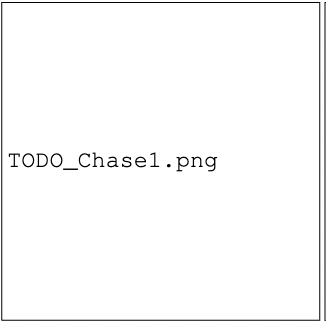
\includegraphics[width=0.5\textwidth,height=7cm,keepaspectratio]{images/TODO_Chase1.png}
    
\includegraphics[width=0.5\textwidth,height=7cm,keepaspectratio]{images/TODO_Chase2.png}
    
    \setbox0=\hbox{\parbox[t]{\textwidth}{
    
    TODO: Your answer for a(ii) here %%%%%% Remove this line in your answer! %%%%%%
    
    %%%%%%% ANSWER ENDS HERE %%%%%%%%%%%%%%%%%%%%%%%%%%%%%%
    }}
    \clipbox{0pt \dimexpr\dp0-12\baselineskip\relax{} 0in 0pt}{\copy0}
    \end{tcolorbox}
    
    \pagebreak
    \item \textbf{[3 points]} 
    LaddObservatory: 
    \href{images/LaddObservatory1.jpg}{LaddObservatory1.jpg} and \href{images/LaddObservatory2.jpg}{LaddObservatory2.jpg}
    \begin{tcolorbox}[colback=white!5!white,colframe=green!75!black]
    
    %%%%%%% ANSWER STARTS HERE %%%%%%%%%%%%%%%%%%%%%%%%%%%%
    %%%%%%% Replace TODO_<placeholder.png> with your picture %%%%%
    
\includegraphics[width=0.5\textwidth,height=7cm,keepaspectratio]{images/TODO_Ladd1.png}
    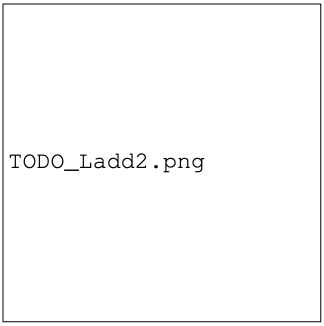
\includegraphics[width=0.5\textwidth,height=7cm,keepaspectratio]{images/TODO_Ladd2.png}
    
    \setbox0=\hbox{\parbox[t]{\textwidth}{
    
    TODO: Your answer for a(iii) here %%%%%% Remove this line in your answer! %%%%%%
    
    %%%%%%% ANSWER ENDS HERE %%%%%%%%%%%%%%%%%%%%%%%%%%%%%%
    }}
    \clipbox{0pt \dimexpr\dp0-12\baselineskip\relax{} 0in 0pt}{\copy0}
    \end{tcolorbox}
\end{enumerate}


\pagebreak
\paragraph{Q3:} \textbf{[9 points]} One use of local feature description and matching is \href{https://www.youtube.com/watch?v=xD88Qs_DZp4}{fingerprint recognition}---please watch the video and note the similarity to our task in this homework. 

Fingerprint recognition uses biometric data---measurements of human biological features that are unique to an individual---to make it convenient to unlock doors or devices quickly and without needing to remember a password. However, given its uniqueness, biometric data may be seen as a greater privacy encroachment upon a person than a password. Further, given the trust that is derived from the uniqueness of biometric data, it may also pose a greater risk of misuse if the data is not secure because the data cannot be changed.

\begin{enumerate}[(a)]
    \item \textbf{[3 points]}
    \begin{tcolorbox}[colback=orange!5!white,colframe=orange!75!black]
    Do you use biometric recognition systems? List them. [If not, list some that people around you use.]
    For one of the systems you use, where is the reference data stored (such as your stored fingerprint), and where and how does the authentication process happen (at a high level)? 
    Try to find the answer online; \href{https://ievoreader.com/how-biometric-data-is-stored/}{this article} may also help. \textbf{[4--6 sentences]}
    \end{tcolorbox}
    
    \begin{tcolorbox}[colback=white!5!white,colframe=green!75!black]
    \setbox0=\hbox{\parbox[t]{\textwidth}{
        %%%%%%% ANSWER STARTS HERE %%%%%%%%%%%%%%%%%%%%%%%%%%%%
            
        TODO: Your answer for (a) here %%%%%% Remove this line in your answer! %%%%%%
            
        %%%%%%% ANSWER ENDS HERE %%%%%%%%%%%%%%%%%%%%%%%%%%%%%%
        }}
    \clipbox{0pt \dimexpr\dp0-12\baselineskip\relax{} 0in 0pt}{\copy0}
    \end{tcolorbox}

    \pagebreak
    \item \textbf{[3 points]}
    \begin{tcolorbox}[colback=orange!5!white,colframe=orange!75!black]
    How might someone use computer vision to steal or spoof your biometric data to gain access? \emph{This could be across reconstruction, recognition, or (re)organization.} \textbf{[3--5 sentences]}
    \end{tcolorbox}

    \begin{tcolorbox}[colback=white!5!white,colframe=green!75!black]
    \setbox0=\hbox{\parbox[t]{\textwidth}{
        %%%%%%% ANSWER STARTS HERE %%%%%%%%%%%%%%%%%%%%%%%%%%%%
            
        TODO: Your answer for (b) here %%%%%% Remove this line in your answer! %%%%%%
            
        %%%%%%% ANSWER ENDS HERE %%%%%%%%%%%%%%%%%%%%%%%%%%%%%%
        }}
    \clipbox{0pt \dimexpr\dp0-12\baselineskip\relax{} 0in 0pt}{\copy0}
    \end{tcolorbox}


    \item
    \textbf{[3 points]}
    \begin{tcolorbox}[colback=orange!5!white,colframe=orange!75!black]
    Biometric recognition systems may not affect all people equally. For a biometric authentication system, define a group of people and describe how they might be affected disproportionately. \textbf{[3--5 sentences]}
    \end{tcolorbox}
    
    \begin{tcolorbox}[colback=white!5!white,colframe=green!75!black]
    \setbox0=\hbox{\parbox[t]{\textwidth}{
        %%%%%%% ANSWER STARTS HERE %%%%%%%%%%%%%%%%%%%%%%%%%%%%
            
        TODO: Your answer for (c) here %%%%%% Remove this line in your answer! %%%%%%
            
        %%%%%%% ANSWER ENDS HERE %%%%%%%%%%%%%%%%%%%%%%%%%%%%%%
        }}
    \clipbox{0pt \dimexpr\dp0-12\baselineskip\relax{} 0in 0pt}{\copy0}
    \end{tcolorbox}
\end{enumerate}

\pagebreak


%%%%%%%%%%%%%%%%%%%%%%%%%%%%%%%%%%%

\paragraph{Q4:} \textbf{[7 points]} Brown University decides to entirely replace passwords with biometric data to authenticate student identity on its computer systems. Given how accurate your feature matching homework 2 code is, Brown asks you to develop the authentication system as your CSCI 1430 final project. Lucky you.

In preparation, you read a previous case about a \href{https://www.vpnmentor.com/blog/report-biostar2-leak/}{biometric data breach}.

\begin{enumerate}[(a)]
    \item \textbf{[3 points]}
    \begin{tcolorbox}[colback=orange!5!white,colframe=orange!75!black]
    How were BioStar 2 storing their fingerprint data? Knowing the computer vision algorithms involved in feature matching, what different processing, features, or storage might you consider instead to decrease the risk of a biometric data breach? \textbf{[4--6 sentences]}
    \end{tcolorbox}

    \begin{tcolorbox}[colback=white!5!white,colframe=green!75!black]
    \setbox0=\hbox{\parbox[t]{\textwidth}{
        %%%%%%% ANSWER STARTS HERE %%%%%%%%%%%%%%%%%%%%%%%%%%%%
            
        TODO: Your answer for (a) here %%%%%% Remove this line in your answer! %%%%%%
            
        %%%%%%% ANSWER ENDS HERE %%%%%%%%%%%%%%%%%%%%%%%%%%%%%%
        }}
    \clipbox{0pt \dimexpr\dp0-15\baselineskip\relax{} 0in 0pt}{\copy0}
    \end{tcolorbox}

    \pagebreak
    \item 
    \textbf{[4 points]}
Even though fingerprints are thought to be unique, we are bound by the accuracy of computer vision systems to detect and recognize that uniqueness.
This may be a challenge for Brown's 10,000 students, let alone a national-scale database such as the FBI's \href{https://www.fbi.gov/services/cjis/fingerprints-and-other-biometrics/ngi}{Next Generation Identification System} that houses over 100 million fingerprints; its Advanced Fingerprint Identification Technology is claimed to be 99.6\% accurate.

Even seemingly high accuracies can create many inaccurate matches with large databases, potentially causing inaccurage judgements in criminal cases. 

    \begin{tcolorbox}[colback=orange!5!white,colframe=orange!75!black]
    In Q2, we asked you to describe issues that might affect correspondence finding in images of natural `human-scale' scenes. Is correspondence finding for fingerprint images an easier problem than for natural images? Why or why not? Think about the variation within each domain of images, the accuracy required, the consequences of matching, and the scope of the application. \textbf{[6--8 sentences]}

    \emph{Refer to the video at the beginning of Q3 and \href{http://biometrics.cse.msu.edu/Presentations/AnilJain_UniquenessOfFingerprints_NAS05.pdf}{the first 15 slides of this deck} for example fingerprint images and additional information.}
    \end{tcolorbox}

    \begin{tcolorbox}[colback=white!5!white,colframe=green!75!black]
    \setbox0=\hbox{\parbox[t]{\textwidth}{
        %%%%%%% ANSWER STARTS HERE %%%%%%%%%%%%%%%%%%%%%%%%%%%%
            
        TODO: Your answer for (b) here %%%%%% Remove this line in your answer! %%%%%%
            
        %%%%%%% ANSWER ENDS HERE %%%%%%%%%%%%%%%%%%%%%%%%%%%%%%
        }}
    \clipbox{0pt \dimexpr\dp0-20\baselineskip\relax{} 0in 0pt}{\copy0}
    \end{tcolorbox}

\end{enumerate}

\pagebreak


%%%%%%%%%%%%%%%%%%%%%%%%%%%%%%%%%%%

% Please leave the pagebreak

\pagebreak
\paragraph{Q5:} \textbf{[3 points]}
As we saw in Q2, the Harris Corner Detector can find feature points for image matching.

To detect these features, the algorithm approximates the strength of any change in the auto-correlation function $E(u, v)$ over shifts $u,v$. We look at the second derivative term in the Taylor series expansion of $E$ to consider the local shape of $E(u, v)$ via the \emph{structure tensor} $M$. Then, we analyze $M$ to determine if that pixel is a corner or not.

\textit{Note:} We expect this conceptual question to require careful study of the lecture slides.

\begin{tcolorbox}[colback=orange!5!white,colframe=orange!75!black]
How do the eigenvalues of the $M$ structure tensor vary with local image brightness, and how might we interpret the eigenvalues geometrically (think `shape')? \textbf{6--8 sentences}
\end{tcolorbox}

\begin{tcolorbox}[colback=white!5!white,colframe=green!75!black]
\setbox0=\hbox{\parbox[t]{\textwidth}{
    %%%%%%% ANSWER STARTS HERE %%%%%%%%%%%%%%%%%%%%%%%%%%%%
        
    TODO: Your answer for Q5 here %%%%%% Remove this line in your answer! %%%%%%
        
    %%%%%%% ANSWER ENDS HERE %%%%%%%%%%%%%%%%%%%%%%%%%%%%%%
    }}
\clipbox{0pt \dimexpr\dp0-18\baselineskip\relax{} 0in 0pt}{\copy0}
\end{tcolorbox}

% Please leave the pagebreak
\pagebreak
\paragraph{Q6:} \textbf{[5 points]}
The SIFT algorithm can extract feature descriptors around feature points. Given a feature point location, the SIFT algorithm converts a 16$\times$16 window around the feature point into a 128$\times$1 feature descriptor via a radial histogram of the gradient magnitudes within the window.


\begin{tcolorbox}[colback=orange!5!white,colframe=orange!75!black]
Write pseudocode \emph{but with correct matrix/array indices} for descriptor extraction.

\emph{Notes:} Do this for just one interest point at one scale; ignore the overall interest point orientation; ignore the Gaussian weighting; ignore all normalization post-processing; ignore image boundaries; ignore sub-pixel interpolation and just pick an arbitrary center within the 16$\times$16 for your feature descriptor.
\end{tcolorbox}

\begin{tcolorbox}[enhanced jigsaw,breakable,pad at break*=1mm,colback=white!5!white,colframe=green!75!black,height fixed for=all]
\begin{python}
# You can assume access to the image, x and y gradients, 
# and their magnitudes/orientations.
image = imread("rara.jpg")
grad_x = filter(image, "sobelX")
grad_y = filter(image, "sobelY")
grad_mag = sqrt(grad_x .^2 + grad_y.^2)
grad_ori = atan2(grad_y, grad_x)

# Takes in a interest point x,y location and returns 
# a feature descriptor
def SIFTdescriptor(x, y)
    descriptor = zeros(128,1)
    
    # TODO: Populate descriptor with the right gradient 
    # magnitudes dependent on the gradient orientations



    
    
    



    
    




    


    return descriptor
\end{python}
%%%%%%%%%%%%%%%%%%%%%%%%%%%%%%%%% 
% DO NOT REMOVE THIS LINE. IT'S TO MAKE SURE PAGE ALIGNMENT IS CORRECT 
\phantom{}
%%%%%%%%%%%%%%%%%%%%%%%%%%%%%%%%% 
\end{tcolorbox}



\pagebreak
\section*{Feedback? (Optional)}
Please help us make the course better. If you have any feedback for this assignment, we'd love to hear it!

\end{document}
